\documentclass[../poliXuniversity_hospital_(USP)_report.tex]{subfiles}
\graphicspath{ {images/}{../images/} } 

\begin{document}
\chapter{Arquitetura do Projeto}

Tanto a Hema Bot, quanto o Golgi Bot e Ciclo Êrgometro seguem a mesma estrutura, que é composta por três núcleos. O Eletrônico, Mecânico e Computacional, cada um responsável pelo desenvolvimento de cada subsistema dos equipamentos e pela integração entre hardware e software de maneira funcional.

\subsection{Sistema Mecânico}

É responsável por realizar toda concepção da estrutura e mecanismos através da modelagem 3D, manufatura de peças, prototipação e manutenção dos projetos. A equipe utiliza e domina softwares CAD de simulação para concepção "virtual", ferramentas como furadeiras, impressoras 3D, esmelhiradeira e entre outras para a manufatura mecânica e também realiza a avaliação e contratação de serviços de usinagem e soldagem. Todas tarefas de prototipagem são realizadas presencialmente no laboratório da ZIMA pelos seus integrantes.

\subsection{Sistema Eletrônico}

Destinado a concepção dos módulos embarcados, fornecimento de energia, sensoriamento e sistema de tração e para isso utiliza Softwares como Altium Designer e NSIM. Além disso é realizado a soldagem das placas de circuito impresso, cabeamento, manutenção eletrônica e compra e contratação de serviços/equipamentos eletrônicos.

\subsection{Sistema Computacional}

Encarregado desenvolver, simular e validar todo software usado nos microcontroladores ou computadores embarcados. Para isso, o dominio de ferramentas de versionamento como Git e GitHub são amplamente utilizados pela equiepe[FOTO] bem como as linguagens C++, Python e frameWorks de simulação como ROS, Rviz e Gazebo[FOTO]. Além de embarcados e simulações, sistemas de interação com usuario também são feitos pela computação[FOTO]. Mais recentemente, a equipe adicionou a área de Desenvolvimento Web e Mobile, responsável pela criação e manutenção do site da zimausp.org[LINK] e do aplicatovo do Hema Bot.


\begin{figure}[h]
\centering
    \caption{Sistema completo - Robô Hospitalar (V2)}
    \centering % para centralizarmos a figura
    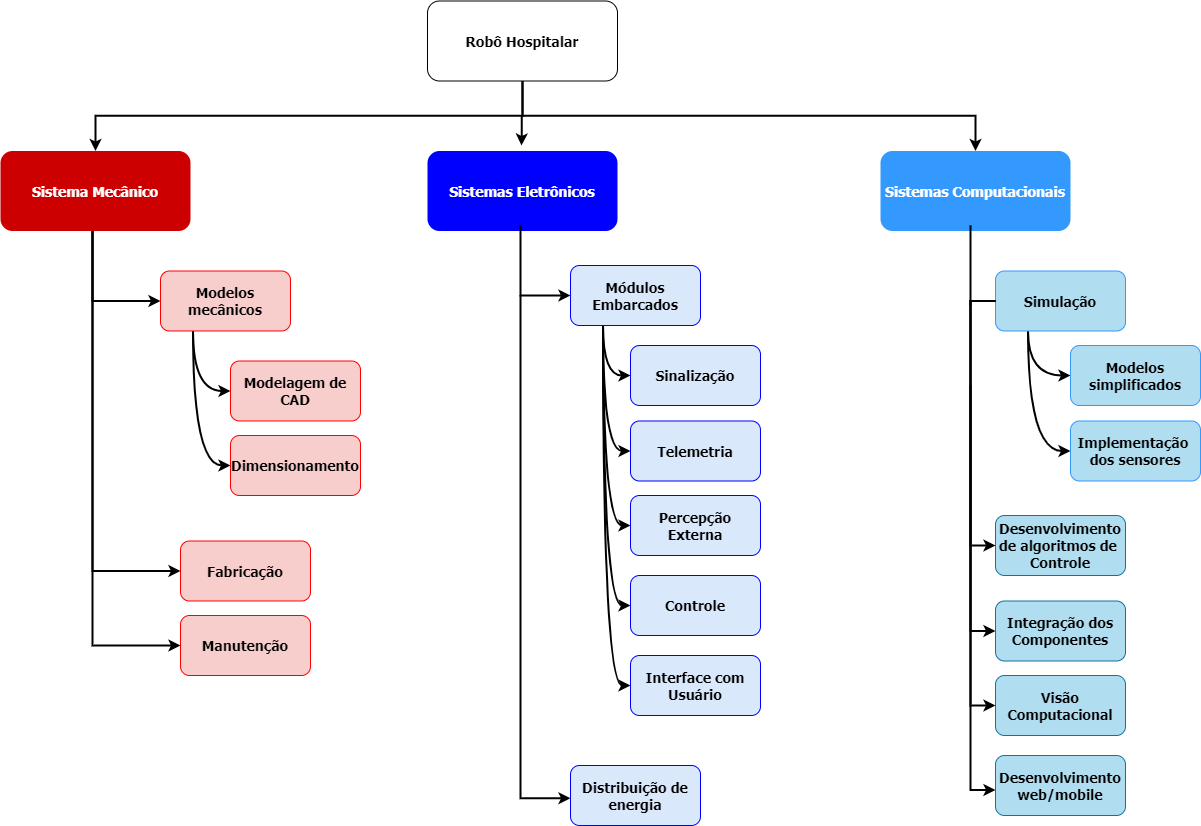
\includegraphics[width=17cm]{sistema_robo.png}
    \caption*{Fonte: Elaborada pelo autor}
    \label{figura:1° Versão Robô Hospitalar}
\end{figure}

\section{Hardware}
Os sistemas eletrônicos do projeto tem como missão, antes de tudo, garantir a locomoção, iluminação, sensoriamento, telemetria modularizada e alimentação elétrica do robô hospitalar, sempre visando a precisão e a segurança. De maneira geral, os sistemas eletrônicos são divididos em duas frentes: Distribuição de energia e Módulos eletrônicos.

A frente de \textbf{distribuição de energia}, até Agosto de 2021, foi pouco explorada. Como um todo no projeto, há somente uma bateria com um tensão contínua elevada para alimentação total do robô e um regulador de tensão chaveado, que é necessário para diminuir a alta tensão da bateria e poder alimentar corretamente os módulos eletrônicos.

Por outro lado, a área dos \textbf{módulos eletrônicos} foi bem trabalhada no último ano. De maneira geral, é dividida em cinco grandes modelos eletrônicos: Sinalização, Percepção Externa, Telemetria, Controle e Interface com Usuário. Cada um desses módulos tem um parte totalmente eletrônica, que é composta por uma placa de circuito impresso, e uma parte do firmware do ESP32 \cite{esp32_datasheet}, o microcontrolador utilizado em cada uma das placas.

Por mais que cada placa tenha seu código único, muitas funções e bibliotecas são reutilizadas, por isso, há uma parte significativa dos códigos que foram feitos como bibliotecas e são usadas em todos os módulos.


\begin{figure}[h]
\centering
    \caption{Sistema Eletronônico - Robô Hospitalar (V2)}
    \centering % para centralizarmos a figura
    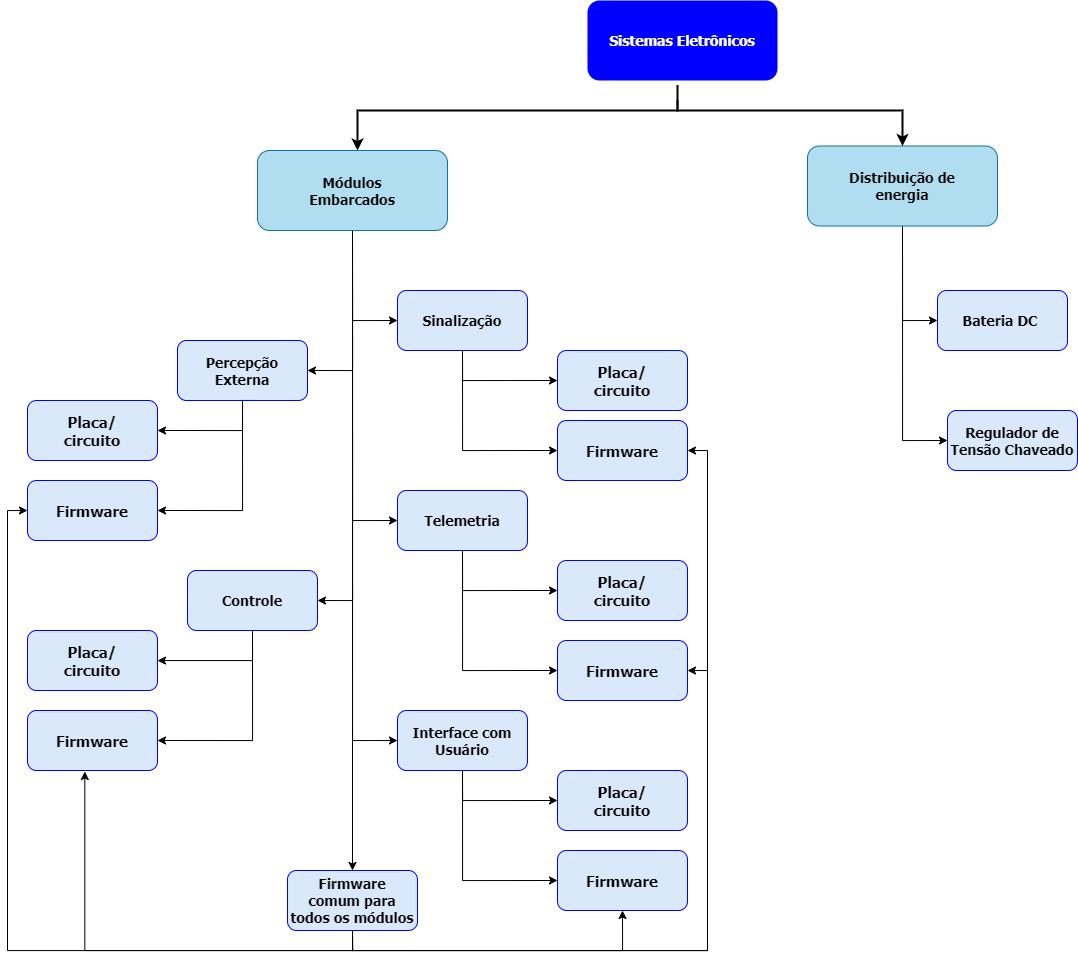
\includegraphics[width=17cm]{sistema_eletronico.png}
    \caption*{Fonte: Elaborada pelo autor}
    \label{figura:1° Versão Robô Hospitalar}
\end{figure}

\section{Software}

A área de computação da equipe, foi sem dúvidas a que mais se desenvolveu nos últimos seis meses. Na primeira versão do robô Hospitalar somente uma pessoa trabalhava, em contrapartida, na segunda versão três pessoas trabalham no software do robô, sendo duas delas inclusivamente para isso. De maneira geral, a confecção do software do robô hospitalar é dividida em cinco grandes frentes: Simulação, Algoritmos de Controle, Integração de Componentes, Visão Computacional e Desenvolvimento Web e  e mobile.

A área de \textbf{Simulação}, feita com gazebo \cite{gazebo21} sem dúvida a melhor desenvolvida e consolidada nos últimos seis meses, que já foi quase que concluída, foi subdividida em três grandes problemas: modelo simplificado do robô, universo de simulação e Implementação de sensores. Esses três problemas já foram devidamente desenvolvidos e hoje em dia sofrem poucas alterações.

A área de \textbf{Desenvolvimento de algoritmos de controle} pode ser subdivida em desenvolver dois grandes problemas: Odometria e Navegação. A odometria consiste em pegar os dados corretamente dos encóderes do robô e navegação em conseguir fazer o robô ir de um ponto a outro de forma autônoma. Ainda está sendo desenvolvida essa parte da equipe, porque é sem dúvida o core de todo o robô.

A área de \textbf{Integração de Componentes} consiste em utilizar a Jetson Nano \cite{jetson21} com os algoritmos desenvolvidos e estabelecer uma conexão com os sistemas embarcados. 

A área de \textbf{Visão computacional} da equipe visa fazer o robô entender alguns objetos de ambientes hospitalares a partir de uma câmera. Por conta de muito trabalho nas outras áreas e a pouca aplicabilidade dela para o projeto hoje, essa parte de desenvolvimento não está com pessoas alocadas oficialmente.

A área de \textbf{Desenvolvimento Web e Mobile}, uma área nova na equipe, que foi adicionada com a entrada de uma nova integrante para o grupo. Essa área está em um momento de pesquisas constantes, porém é bem promissora para um futuro breve.  


\begin{figure}[h]
\centering
    \caption{Sistema Computacional - Robô Hospitalar (V2)}
    \centering % para centralizarmos a figura
    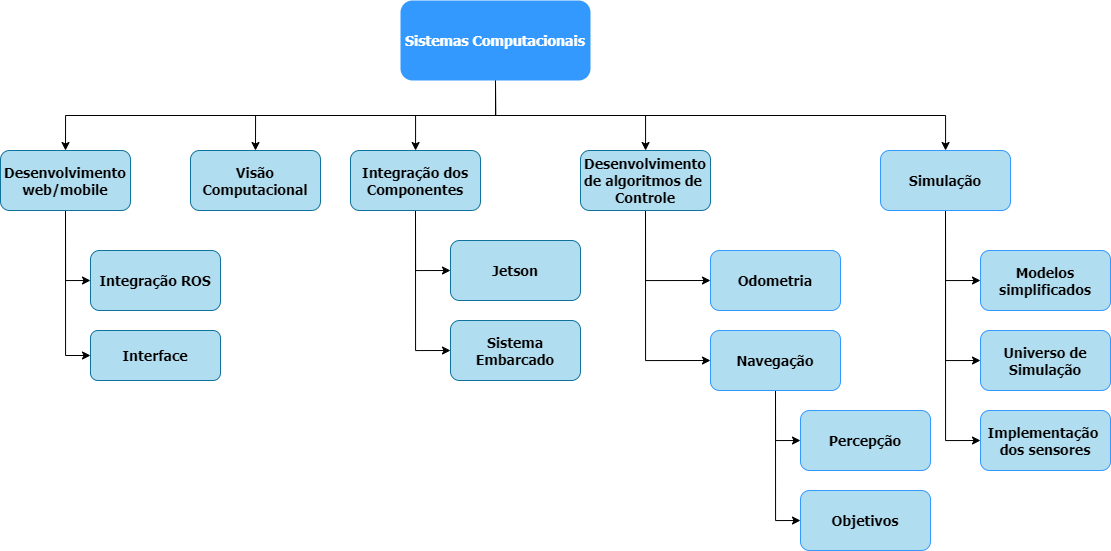
\includegraphics[width=17cm]{sistema_computacional.png}
    \caption*{Fonte: Elaborada pelo autor}
    \label{figura:1° Versão Robô Hospitalar}
\end{figure}


\end{document}